\documentclass[12pt,a4paper]{article}

% Modele de rapport de stage et conseils de redaction, mise en page...
% L. Bellon, avril 2010

% definition des marges du document
\setlength{\topmargin}{0cm}
\setlength{\headheight}{0.4cm}
\setlength{\headsep}{0.8cm}
\setlength{\footskip}{1cm}
\setlength{\textwidth}{17cm}
\setlength{\textheight}{25cm}
\setlength{\voffset}{-1.5cm}
\setlength{\hoffset}{-0.5cm}
\setlength{\oddsidemargin}{0cm}
\setlength{\evensidemargin}{0cm}

% quelques package utiles
\usepackage{graphicx} % inclusion des figures
\usepackage{epstopdf} %inclusion .eps pour pdflatex

\usepackage{listings}
\usepackage{amsmath} % collection de symboles mathematiques
\usepackage{amssymb} % collection de symboles mathematiques

\usepackage{multicol,caption, subcaption}

\usepackage[utf8]{inputenc}
\usepackage[T1]{fontenc} % codage moderne des caracteres sous Latex

\usepackage[english]{babel}
\usepackage{natbib}

\usepackage{tabularx} % gestion avancee des tableaux

\usepackage{psfrag} % remplacement du texte d'une figure ps par du texte latex
\usepackage{siunitx} % units
\usepackage{physics} % to write physical equations

\usepackage{color} % gestion de differentes couleurs

\definecolor{linkcolor}{rgb}{0.3,0,0.2} % definition de la couleur des liens pdf
\usepackage[ pdftex,colorlinks=true,
pdfstartview=FitV,
linkcolor= linkcolor,
citecolor= linkcolor,
urlcolor= linkcolor,
hyperindex=true,
hyperfigures=false]
{hyperref} % fichiers pdf 'intelligents', avec des liens entre les references, etc.

\usepackage{fancyhdr} % entetes et pieds de pages personnalises

% commande de deplacement d'un objet
\newcommand{\drawat}[3]{\makebox[0pt][l]{\raisebox{#2}{\hspace*{#1}#3}}}

\usepackage{color}

\definecolor{mygreen}{rgb}{0,0.6,0}
\definecolor{mygray}{rgb}{0.5,0.5,0.5}
\definecolor{mymauve}{rgb}{0.58,0,0.82}

\lstset{ %
  backgroundcolor=\color{white},   % choose the background color; you must add \usepackage{color} or \usepackage{xcolor}
  basicstyle=\footnotesize,        % the size of the fonts that are used for the code
  breakatwhitespace=false,         % sets if automatic breaks should only happen at whitespace
  breaklines=true,                 % sets automatic line breaking
  captionpos=b,                    % sets the caption-position to bottom
  commentstyle=\color{mygreen},    % comment style
  deletekeywords={...},            % if you want to delete keywords from the given language
  escapeinside={\%*}{*)},          % if you want to add LaTeX within your code
  extendedchars=true,              % lets you use non-ASCII characters; for 8-bits encodings only, does not work with UTF-8
  frame=single,                    % adds a frame around the code
  keepspaces=true,                 % keeps spaces in text, useful for keeping indentation of code (possibly needs columns=flexible)
  keywordstyle=\color{blue},       % keyword style
  language=Octave,                 % the language of the code
  otherkeywords={*,...},            % if you want to add more keywords to the set
  numbers=left,                    % where to put the line-numbers; possible values are (none, left, right)
  numbersep=5pt,                   % how far the line-numbers are from the code
  numberstyle=\tiny\color{mygray}, % the style that is used for the line-numbers
  rulecolor=\color{black},         % if not set, the frame-color may be changed on line-breaks within not-black text (e.g. comments (green here))
  showspaces=false,                % show spaces everywhere adding particular underscores; it overrides 'showstringspaces'
  showstringspaces=false,          % underline spaces within strings only
  showtabs=false,                  % show tabs within strings adding particular underscores
  stepnumber=2,                    % the step between two line-numbers. If it's 1, each line will be numbered
  stringstyle=\color{mymauve},     % string literal style
  tabsize=2,                       % sets default tabsize to 2 spaces
  title=\lstname                   % show the filename of files included with \lstinputlisting; also try caption instead of title
}

\newcommand{\degree}{^{\circ}}
\newcommand{\cred}{\color{red}}

\graphicspath{{Figures/}} %Position of figures, pictures, etc

% definition de l'entete et du pied de page
\pagestyle{fancy}
\fancyhead[L]{\scriptsize \textsc{Field work: blabla TODO}}
\fancyhead[R]{\scriptsize \textsc{Romain Caneill}}
\fancyfoot[C]{ \thepage}

\begin{document}
% Pour faciliter la mise en forme de la page du titre, on supprime l'indentation automatique en debut de paragraphe
\setlength{\parindent}{0pt}

% Pas d'en-tete ni de pied pour la premiere page
\thispagestyle{empty}

\begin{minipage}{0.4\paperwidth}
  {\sc Physical Oceanography} \\
{\it Göteborgs universitet}\\
{\it Institutionen för marina vetenskaper}
\end{minipage}
\begin{minipage}{0.3\paperwidth}
  
\includegraphics[height=2.9cm]{gu}
\end{minipage}
\begin{minipage}{0.2\paperwidth}
  Romain Caneill\\
  PhD Student
\end{minipage}

\begin{center}
\vspace{.3cm}

\rule[5pt]{10cm}{0.5pt}
\vspace{10pt}

\textbf{\Large Find a title.}
\vspace{8pt}

\rule{10cm}{0.5pt}

\vspace{.3cm}

\parbox{15cm}{\small
\textbf{Abstract}: \it TODO
} %fin de la commande \parbox du resume

\vspace{0.5cm}

\parbox{15cm}{
\textbf{Keywords}: \it CTD, Field work, TODO
} %fin de la commande \parbox des mots clefs

\end{center}

\newpage

% Premiere page du rapport
\setcounter{page}{1}
\setlength\parindent{24pt}

\newpage

\tableofcontents

\newpage

\section{\label{sec_intro}Introduction}

TODO find references about fjords, skagerrak

\section{Materials and methods}
\subsection{Presentation of the field work and data acquisition}

This report focuses on a field work that has been conducted on December 2018, the
10th and 11th, as part of the course OC4920 of the University of Gothenburg.
Two days have been spent on two ships, the Skagerrak and the Trygve.
Both ships had fully equipped CTD, with temperature, salinity, and oxygen concentration
sensors. Some other variables have been recorded but not discussed on this
report. Niskins bottle have been used for the oxygen calibration on board of
the Skagerrak.

We got more than 50 casts, covering the fjord with a very good spatial coverage.
We also made 3 mooring measurements, setting the CTD at a certain depth
for 30 minutes, recording the temporal variations instead of the
spatial variations.
Figure~\ref{fig:stations} presents the position of the Gullman Fjord, on the western
coast of Sweden, as well as the position of the CTD casts.

\begin{figure}
  \centering
  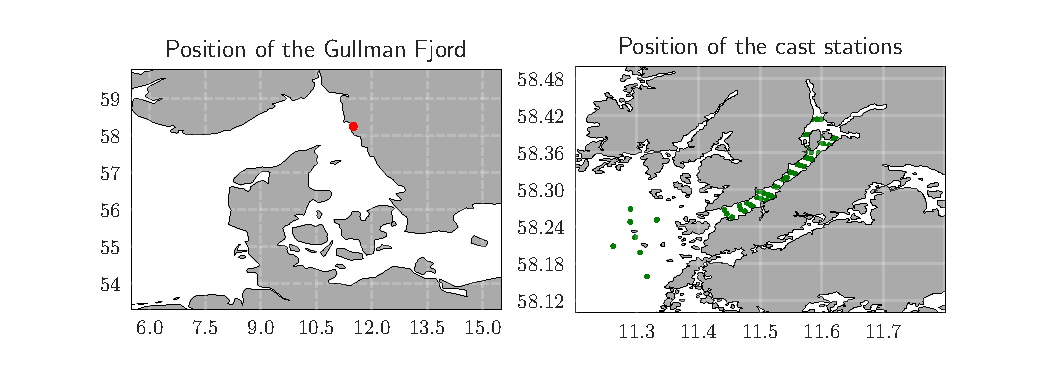
\includegraphics{stations}
  \caption{\label{fig:stations}Situation of the Gullman Fjord (red dot) and position
    of the CTD casts (green dots).}
\end{figure}

\subsection{Data processing}
For a better readability, we will refer to potential temperature as temperature
and to absolute salinity as salinity.
If needed, we will explicitly use the term {\it in situ} to refer to
measured temperature and salinity.

To ensure coherence in the whole dataset and between the two ships,
all the data have been regridded on a 1 meter grid, from 0 to 119 meters depth.
Depths without any measurement points have been filled with NaN.

\paragraph{Processing}
Using the library provided by TEOS-10 \citep{gsw}, {\it in situ} temperatures and practical
salinities have been converted to potential temperature and absolute salinity.
Potential density anomaly has also been derived.

\paragraph{Calibration}
One cast has been conducted at the same position with the two ships each day,
so that all the measured variables can be calibrated between the two datasets.
The Skagerrak data have been chosen as reference data, because of a more
recent recalibration of the CTD sensors than the Trygve sensors.
After a linear regression between Trygve and Skagerrak calibration profiles
under the thermocline, the coefficients have been used to recalibrate
Trygve profiles for each day.
See Table~\ref{tab:calib} for the used coefficients.


\subsection{Turner angle}
One way to estimate the role of the salinity and the temperature on the stratification
is to use the Turner angle.
\citep{ruddick1983, johnson2012}

\subsection{Geostrophy TODO compute}
\subsection{Profile fitting and layers}
Temperature profiles in the fjord all look very similar, with
\begin{inparaenum}
\item an upper thermocline;
\item a warm water mass;
\item a lower thermocline;
\item the lowest layer where temperature is approximately constant.
\end{inparaenum}
It is not easy to compute the depth of these layer by using a threshold (on the
value or on the gradient) due to the irregularities of the temperature.
Inspired by the work of \cite{pauthenet2017}, we decided to approximate
the profiles with a function and then extract the layers information from the
functions properties. As the studied profiles have all the same shapes,
we used a mutli-linear fit, fitting the 4 layers.
The parameters of the fitted function are the depths and the temperatures
of the interface between each layers. We considered that for the lowest layer,
the fitted temperature will be a constant. An {\it a priori} model was set
for these 8 parameters, with values set by eye to be a good candidate.
Table~\ref{tab:apriori} in Appendix presents the parameters. The least squares
approximation has been used to find the best parameters.
For the profiles that are not deep enough, only the part where data are present
has been used for the least squares method. The {\it a priori} model
has been set for the lower part, with a confidence flag set to 0.
Figure~\ref{fig:fit} presents two examples of profiles: one where the 4 layers
are present and one where the fjord was not deep enough, so only
the upper layer is fitted.

\begin{figure}
  \centering
  \includegraphics{{explainProfFit}}
  \caption{\label{fig:fit}Profile fitting with a multi-linear function.
    The measured profiles are plotted in green, the fitted functions in blue,
    and the red crosses represent depth and temperature at the interfaces
    between the different layers. On the right plot, the fit corresponds to the
    {\it a priori} model for the two lowest interfaces.}
\end{figure}

\paragraph{No sub-mesoscale heat fluxes because no mixed layer}

\section{Results}

\paragraph{T-S diagram}
see figure \ref{fig:ts}

we recognize Skagerrak and Kattegat water \citep{bjork2003,gustafsson1996}

Kattegat salinity 15/20(depending on the source)-25

Skagerrak salinity between 33 (surface) to 35 (100m depth)

\begin{figure}
  \centering
  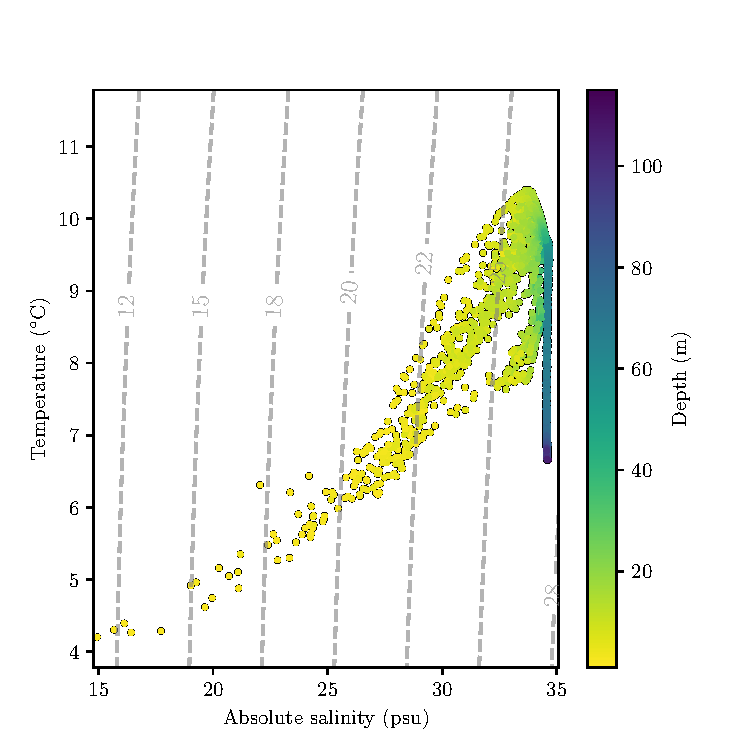
\includegraphics{ts}
  \caption{\label{fig:ts}T-S diagram}
\end{figure}

\paragraph{warm water layer}
warm water in the fjord, see mean depth, std depth, mean T and S, see spatial
distribution

\paragraph{strong halocline}

\paragraph{Turner angle}
\begin{figure}
  \centering
  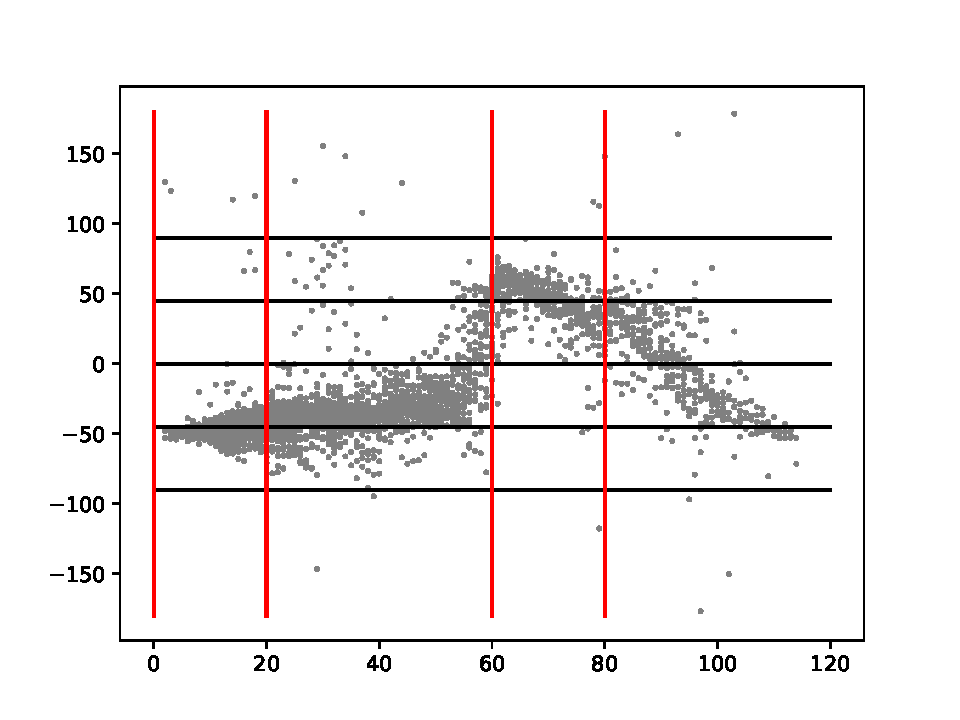
\includegraphics{turner}
  \caption{\label{fig:turner}Turner angle as a function of depth.}
\end{figure}

\paragraph{Geostrophy}
What is happening here?

\paragraph{Upwelling event? Mixing?}
\citep{arneborg2003}

\section{Discussion}

TODO

fitting of the profile, using spline could be better. but here maybe not necessary. 

\section{Conclusion}

See what is the context\\
What we did\\
What we showed/saw\\
What is the conclusion

%\newpage

\bibliographystyle{../Biblio/agufull08}
\bibliography{../Biblio/biblio}

\newpage

%\renewcommand\thefigure{\thesection.\arabic{figure}}
\appendix
\setcounter{figure}{0}

\section{Complementary data and figures}

\begin{table}[h]
  \centering
  \begin{tabular}{|l|c|r|}
    \hline
    Depth (m) & Temperature ($\degree$C) & Comment \\
    \hline
    0 & 5 & Surface\\
    20 & 10 & Bottom of the upper thermocline / top of the warm water\\
    60 & 9 & Bottom of the warm water / top of the lower thermocline\\
    80 & 7 & Bottom of the lower thermocline / top of the lowest layer\\
    \hline
  \end{tabular}
  \caption{\label{tab:apriori}Values of the {\it a priori} model for the multi-linear fit.}
\end{table}

\begin{table}[h]
  \centering
  Temperature\\
  \begin{tabular}{|l|c|c|}
    \hline
    Date & $a_T$ & $b_T$ \\
    \hline
    2018-12-10 & 0.9938598212928323461 & 0.07856246515108189499\\
    2018-12-11 & 1.006636216123387273  & -0.09514920786826941423\\
    \hline
  \end{tabular}
  
  \vspace{.5cm}
  Salinity\\
  \begin{tabular}{|l|c|c|}
    \hline
    Date & $a_S$ & $a_S$ \\
    \hline
    2018-12-10 & 0.8453445700814513630 & 5.276859099581269419\\
    2018-12-11 & 0.8190729895351881451 & 6.231978296168669829\\
    \hline
  \end{tabular}
  \caption{\label{tab:calib}Regression coefficients, the calibration has the following
    shape:
    ${X_{Trygve} = a_X \cdot X_{Skagerrak} + b_X}$, with $X$
    the temperature or the salinity.}
\end{table}

TODO

ALL THE FIGURES I WANT TO PUT ON THE REPORT

For all profiles, put 2 different color for offshore and fjord
\begin{figure}[h]
  \centering
  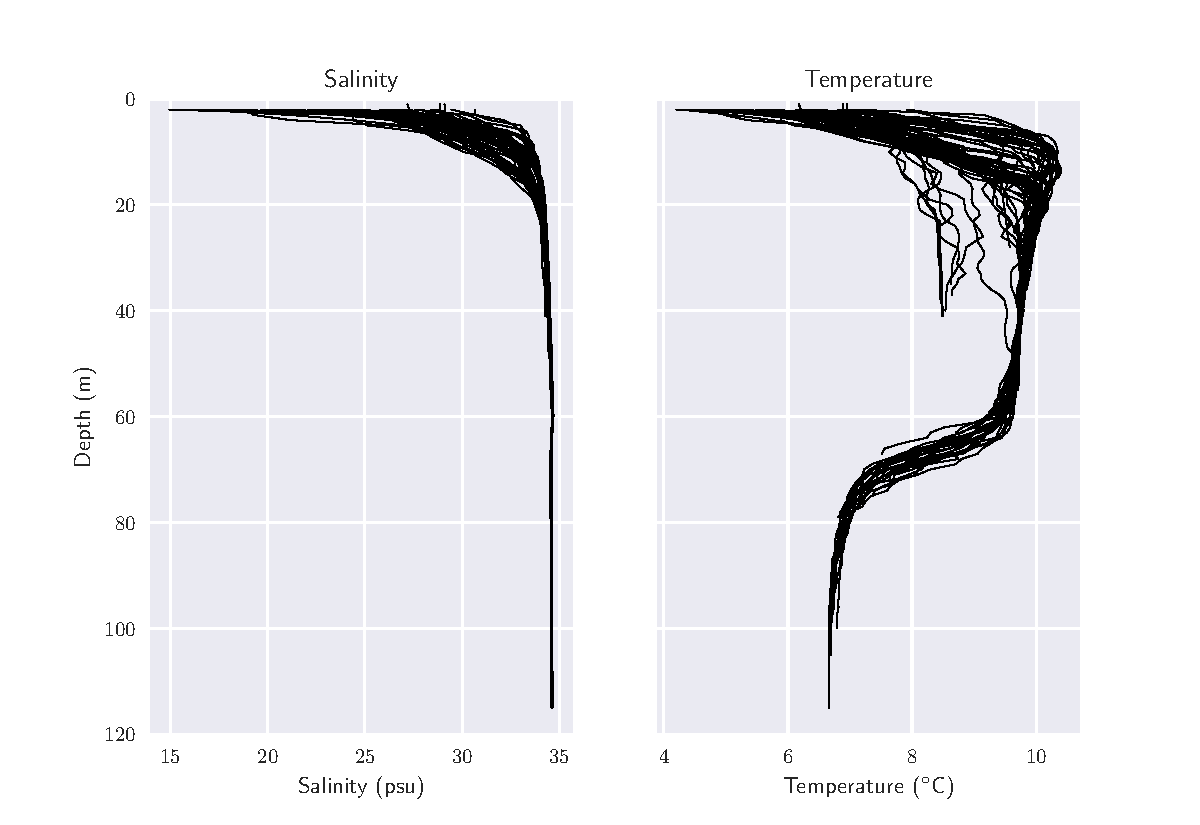
\includegraphics[width=.3\textwidth]{profileTot}
  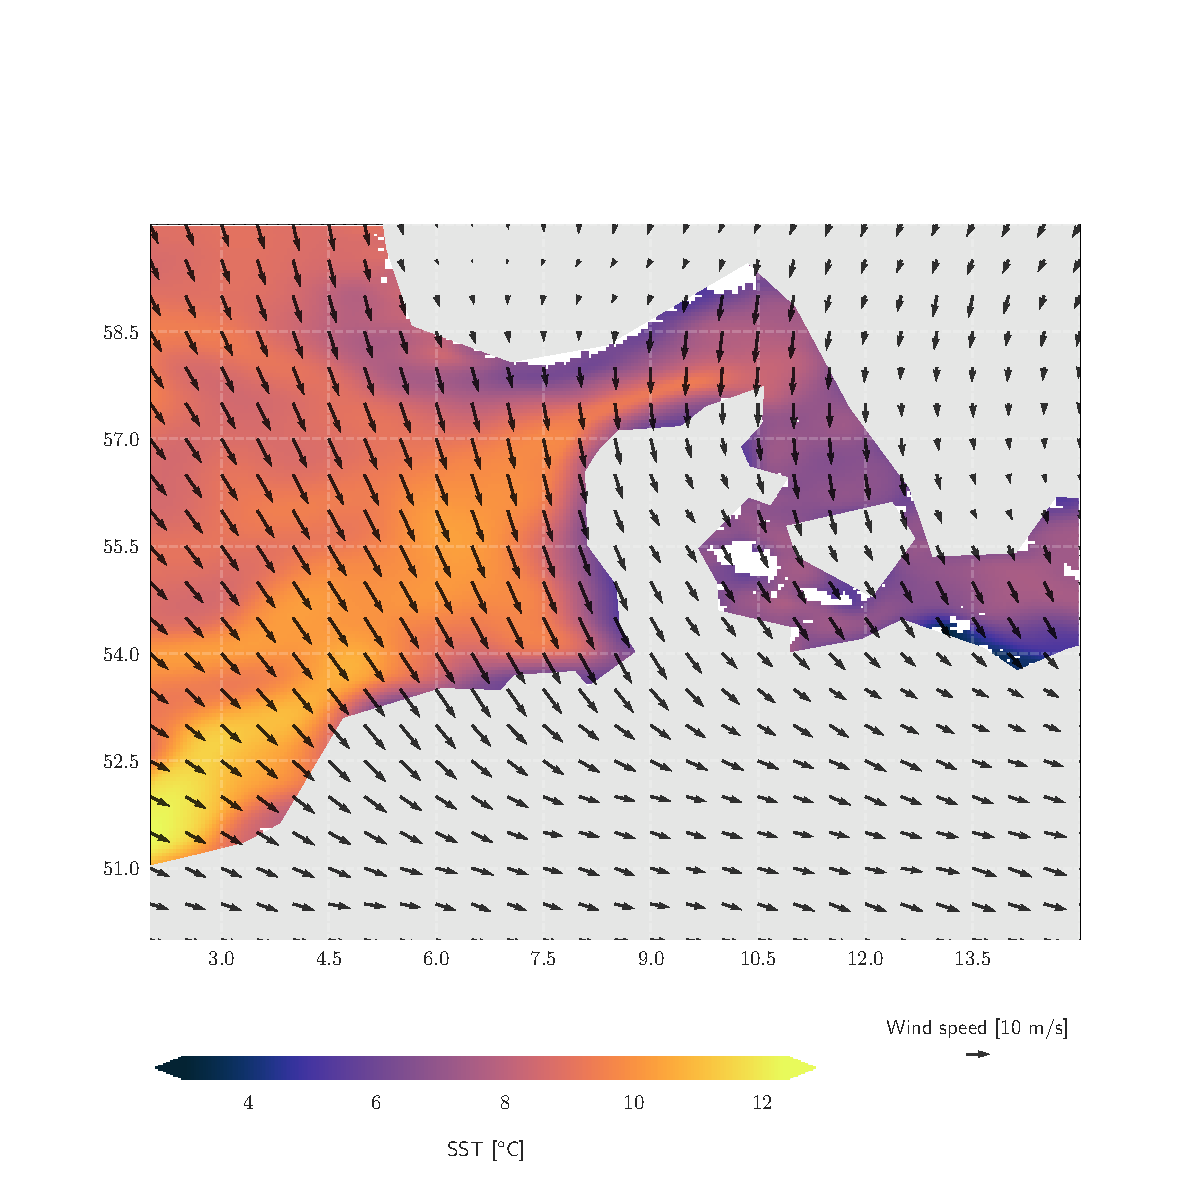
\includegraphics[width=.3\textwidth]{synoptic_conditions}
  \includegraphics[width=.3\textwidth]{{sal_20181210}}
  \includegraphics[width=.3\textwidth]{{layer_bottom_of_thermocline}}
  \includegraphics[width=.3\textwidth]{{layer_bottom_of_warm_water}}
  \includegraphics[width=.3\textwidth]{{transect_0}}
  \includegraphics[width=.3\textwidth]{{transect_2}}
\end{figure}

\end{document}
